\documentclass{standalone}
\usepackage{tikz}
\usetikzlibrary{patterns, positioning}


\begin{document}
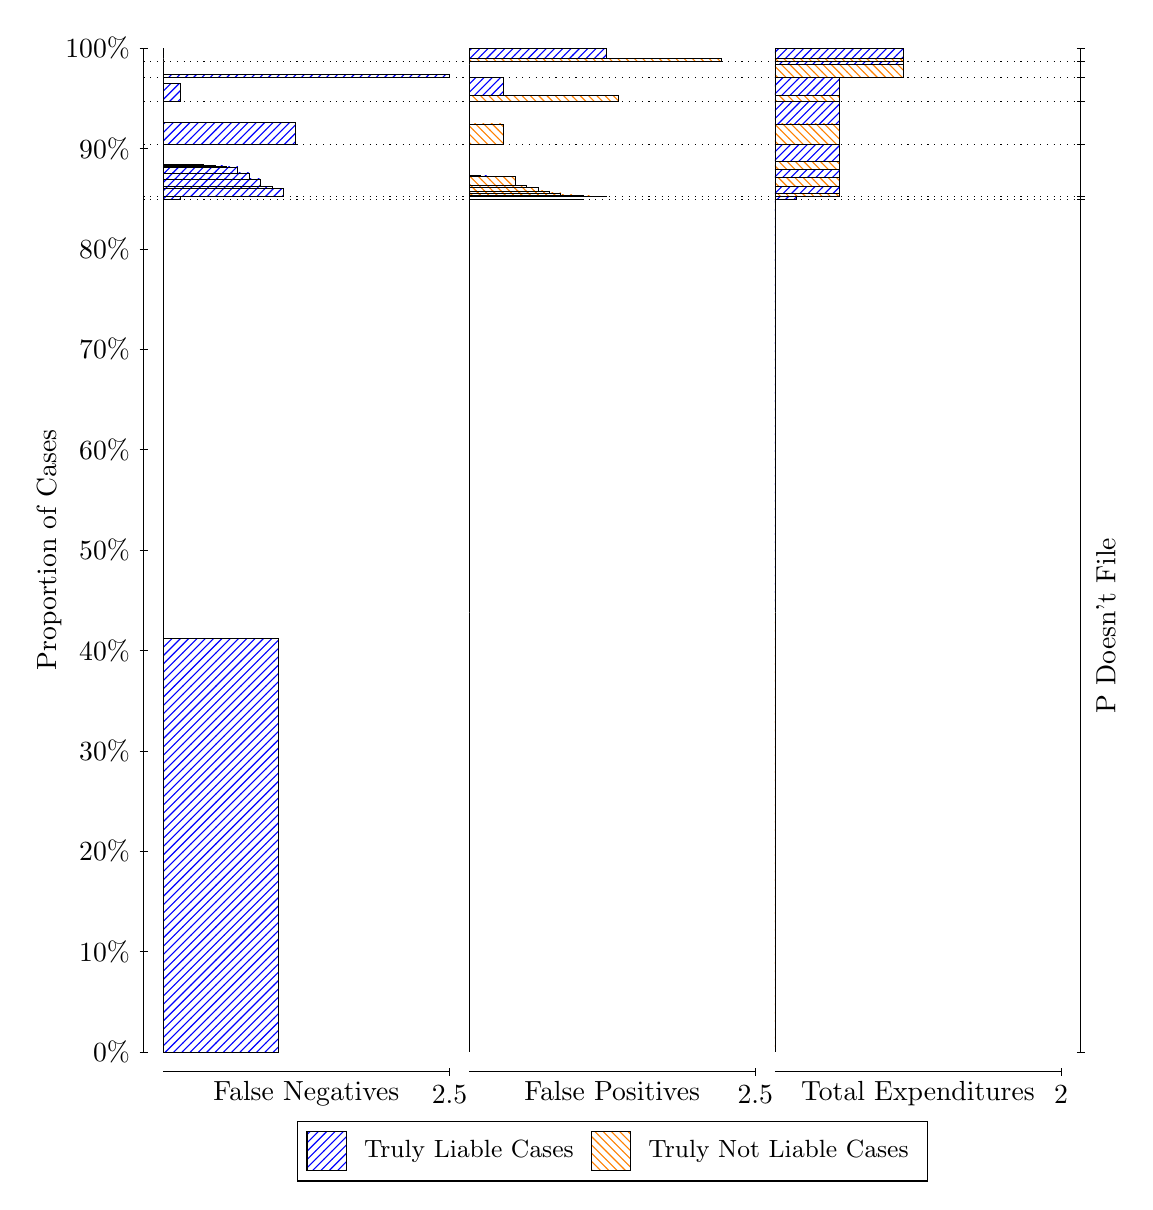
\begin{tikzpicture}
\draw[black, very thin] (1.5,1.75) -- (1.5,14.5);
\node[rotate=90, text=black, anchor=center] at (0.3, 8.125) {Proportion of Cases};
\draw[black, very thin] (1.45,1.75) -- (1.55,1.75);
\node[text=black, anchor=east] at (1.45, 1.75) {0\%};
\draw[black, very thin] (1.45,3.025) -- (1.55,3.025);
\node[text=black, anchor=east] at (1.45, 3.025) {10\%};
\draw[black, very thin] (1.45,4.3) -- (1.55,4.3);
\node[text=black, anchor=east] at (1.45, 4.3) {20\%};
\draw[black, very thin] (1.45,5.575) -- (1.55,5.575);
\node[text=black, anchor=east] at (1.45, 5.575) {30\%};
\draw[black, very thin] (1.45,6.85) -- (1.55,6.85);
\node[text=black, anchor=east] at (1.45, 6.85) {40\%};
\draw[black, very thin] (1.45,8.125) -- (1.55,8.125);
\node[text=black, anchor=east] at (1.45, 8.125) {50\%};
\draw[black, very thin] (1.45,9.4) -- (1.55,9.4);
\node[text=black, anchor=east] at (1.45, 9.4) {60\%};
\draw[black, very thin] (1.45,10.675) -- (1.55,10.675);
\node[text=black, anchor=east] at (1.45, 10.675) {70\%};
\draw[black, very thin] (1.45,11.95) -- (1.55,11.95);
\node[text=black, anchor=east] at (1.45, 11.95) {80\%};
\draw[black, very thin] (1.45,13.225) -- (1.55,13.225);
\node[text=black, anchor=east] at (1.45, 13.225) {90\%};
\draw[black, very thin] (1.45,14.5) -- (1.55,14.5);
\node[text=black, anchor=east] at (1.45, 14.5) {100\%};

\draw[black, very thin] (13.4,1.75) -- (13.4,14.5);
\draw[black, very thin] (13.35,1.75) -- (13.45,1.75);
\node[anchor=west] at (13.35, 1.75) {};
\draw[black, very thin] (13.35,12.577) -- (13.45,12.577);
\node[anchor=west] at (13.35, 12.577) {};
\draw[black, very thin] (13.35,12.617) -- (13.45,12.617);
\node[anchor=west] at (13.35, 12.617) {};
\draw[black, very thin] (13.35,13.276) -- (13.45,13.276);
\node[anchor=west] at (13.35, 13.276) {};
\draw[black, very thin] (13.35,13.818) -- (13.45,13.818);
\node[anchor=west] at (13.35, 13.818) {};
\draw[black, very thin] (13.35,14.13) -- (13.45,14.13);
\node[anchor=west] at (13.35, 14.13) {};
\draw[black, very thin] (13.35,14.331) -- (13.45,14.331);
\node[anchor=west] at (13.35, 14.331) {};
\draw[black, very thin] (13.35,14.5) -- (13.45,14.5);
\node[anchor=west] at (13.35, 14.5) {};

\draw[black, very thin, pattern color=blue, pattern=north east lines] (1.75,1.75) rectangle (3.2033,6.9983);
\draw[black, very thin, pattern color=orange, pattern=north west lines] (1.75,6.9983) rectangle (1.75,12.577);
\draw[black, very thin, pattern color=blue, pattern=north east lines] (1.75,12.577) rectangle (1.968,12.613);
\draw[black, very thin, pattern color=orange, pattern=north west lines] (1.75,12.613) rectangle (1.75,12.617);
\draw[black, very thin, pattern color=blue, pattern=north east lines] (1.75,12.617) rectangle (3.276,12.719);
\draw[black, very thin, pattern color=blue, pattern=north east lines] (1.75,12.719) rectangle (3.1307,12.746);
\draw[black, very thin, pattern color=blue, pattern=north east lines] (1.75,12.746) rectangle (2.9853,12.837);
\draw[black, very thin, pattern color=blue, pattern=north east lines] (1.75,12.837) rectangle (2.84,12.914);
\draw[black, very thin, pattern color=blue, pattern=north east lines] (1.75,12.914) rectangle (2.6947,12.991);
\draw[black, very thin, pattern color=blue, pattern=north east lines] (1.75,12.991) rectangle (2.5493,13.002);
\draw[black, very thin, pattern color=blue, pattern=north east lines] (1.75,13.002) rectangle (2.404,13.013);
\draw[black, very thin, pattern color=blue, pattern=north east lines] (1.75,13.013) rectangle (2.2587,13.018);
\draw[black, very thin, pattern color=blue, pattern=north east lines] (1.75,13.018) rectangle (2.1133,13.023);
\draw[black, very thin, pattern color=orange, pattern=north west lines] (1.75,13.023) rectangle (1.75,13.276);
\draw[black, very thin, pattern color=blue, pattern=north east lines] (1.75,13.276) rectangle (3.4213,13.556);
\draw[black, very thin, pattern color=orange, pattern=north west lines] (1.75,13.556) rectangle (1.75,13.818);
\draw[black, very thin, pattern color=blue, pattern=north east lines] (1.75,13.818) rectangle (1.968,14.053);
\draw[black, very thin, pattern color=orange, pattern=north west lines] (1.75,14.053) rectangle (1.75,14.13);
\draw[black, very thin, pattern color=blue, pattern=north east lines] (1.75,14.13) rectangle (5.3833,14.169);
\draw[black, very thin, pattern color=orange, pattern=north west lines] (1.75,14.169) rectangle (1.75,14.331);
\draw[black, very thin, pattern color=orange, pattern=north west lines] (1.75,14.331) rectangle (1.75,14.37);
\draw[black, very thin, pattern color=blue, pattern=north east lines] (1.75,14.37) rectangle (1.75,14.5);
\draw[black, very thin, pattern color=orange, pattern=north west lines] (5.6333,1.75) rectangle (5.6333,7.329);
\draw[black, very thin, pattern color=blue, pattern=north east lines] (5.6333,7.329) rectangle (5.6333,12.577);
\draw[black, very thin, pattern color=orange, pattern=north west lines] (5.6333,12.577) rectangle (7.0867,12.581);
\draw[black, very thin, pattern color=blue, pattern=north east lines] (5.6333,12.581) rectangle (5.6333,12.617);
\draw[black, very thin, pattern color=orange, pattern=north west lines] (5.6333,12.617) rectangle (7.3773,12.62);
\draw[black, very thin, pattern color=orange, pattern=north west lines] (5.6333,12.62) rectangle (7.232,12.623);
\draw[black, very thin, pattern color=orange, pattern=north west lines] (5.6333,12.623) rectangle (7.0867,12.628);
\draw[black, very thin, pattern color=orange, pattern=north west lines] (5.6333,12.628) rectangle (6.9413,12.635);
\draw[black, very thin, pattern color=orange, pattern=north west lines] (5.6333,12.635) rectangle (6.796,12.661);
\draw[black, very thin, pattern color=orange, pattern=north west lines] (5.6333,12.661) rectangle (6.6507,12.687);
\draw[black, very thin, pattern color=orange, pattern=north west lines] (5.6333,12.687) rectangle (6.5053,12.734);
\draw[black, very thin, pattern color=orange, pattern=north west lines] (5.6333,12.734) rectangle (6.36,12.759);
\draw[black, very thin, pattern color=orange, pattern=north west lines] (5.6333,12.759) rectangle (6.2147,12.87);
\draw[black, very thin, pattern color=blue, pattern=north east lines] (5.6333,12.87) rectangle (5.924,12.875);
\draw[black, very thin, pattern color=blue, pattern=north east lines] (5.6333,12.875) rectangle (5.7787,12.88);
\draw[black, very thin, pattern color=blue, pattern=north east lines] (5.6333,12.88) rectangle (5.6333,13.276);
\draw[black, very thin, pattern color=orange, pattern=north west lines] (5.6333,13.276) rectangle (6.0693,13.538);
\draw[black, very thin, pattern color=blue, pattern=north east lines] (5.6333,13.538) rectangle (5.6333,13.818);
\draw[black, very thin, pattern color=orange, pattern=north west lines] (5.6333,13.818) rectangle (7.5227,13.895);
\draw[black, very thin, pattern color=blue, pattern=north east lines] (5.6333,13.895) rectangle (6.0693,14.13);
\draw[black, very thin, pattern color=orange, pattern=north west lines] (5.6333,14.13) rectangle (5.6333,14.292);
\draw[black, very thin, pattern color=blue, pattern=north east lines] (5.6333,14.292) rectangle (5.6333,14.331);
\draw[black, very thin, pattern color=orange, pattern=north west lines] (5.6333,14.331) rectangle (8.8307,14.37);
\draw[black, very thin, pattern color=blue, pattern=north east lines] (5.6333,14.37) rectangle (7.3773,14.5);
\draw[black, very thin, pattern color=orange, pattern=north west lines] (9.5167,1.75) rectangle (9.5167,7.329);
\draw[black, very thin, pattern color=blue, pattern=north east lines] (9.5167,7.329) rectangle (9.5167,12.577);
\draw[black, very thin, pattern color=orange, pattern=north west lines] (9.5167,12.577) rectangle (9.7892,12.581);
\draw[black, very thin, pattern color=blue, pattern=north east lines] (9.5167,12.581) rectangle (9.7892,12.617);
\draw[black, very thin, pattern color=orange, pattern=north west lines] (9.5167,12.617) rectangle (10.334,12.652);
\draw[black, very thin, pattern color=blue, pattern=north east lines] (9.5167,12.652) rectangle (10.334,12.745);
\draw[black, very thin, pattern color=orange, pattern=north west lines] (9.5167,12.745) rectangle (10.334,12.856);
\draw[black, very thin, pattern color=blue, pattern=north east lines] (9.5167,12.856) rectangle (10.334,12.959);
\draw[black, very thin, pattern color=orange, pattern=north west lines] (9.5167,12.959) rectangle (10.334,13.065);
\draw[black, very thin, pattern color=blue, pattern=north east lines] (9.5167,13.065) rectangle (10.334,13.276);
\draw[black, very thin, pattern color=orange, pattern=north west lines] (9.5167,13.276) rectangle (10.334,13.538);
\draw[black, very thin, pattern color=blue, pattern=north east lines] (9.5167,13.538) rectangle (10.334,13.818);
\draw[black, very thin, pattern color=orange, pattern=north west lines] (9.5167,13.818) rectangle (10.334,13.895);
\draw[black, very thin, pattern color=blue, pattern=north east lines] (9.5167,13.895) rectangle (10.334,14.13);
\draw[black, very thin, pattern color=orange, pattern=north west lines] (9.5167,14.13) rectangle (11.152,14.292);
\draw[black, very thin, pattern color=blue, pattern=north east lines] (9.5167,14.292) rectangle (11.152,14.331);
\draw[black, very thin, pattern color=orange, pattern=north west lines] (9.5167,14.331) rectangle (11.152,14.37);
\draw[black, very thin, pattern color=blue, pattern=north east lines] (9.5167,14.37) rectangle (11.152,14.5);
\draw[black, dotted] (1.5,12.577) -- (13.4,12.577);
\draw[black, dotted] (1.5,12.617) -- (13.4,12.617);
\draw[black, dotted] (1.5,13.276) -- (13.4,13.276);
\draw[black, dotted] (1.5,13.818) -- (13.4,13.818);
\draw[black, dotted] (1.5,14.13) -- (13.4,14.13);
\draw[black, dotted] (1.5,14.331) -- (13.4,14.331);
\draw[black, very thin] (1.75,1.5) -- (5.3833,1.5);
\node[text=black, anchor=north] at (3.5667, 1.5) {False Negatives};
\draw[black, very thin] (5.3833,1.45) -- (5.3833,1.55);
\node[text=black, anchor=north] at (5.3833, 1.45) {2.5};

\draw[black, very thin] (5.6333,1.5) -- (9.2667,1.5);
\node[text=black, anchor=north] at (7.45, 1.5) {False Positives};
\draw[black, very thin] (9.2667,1.45) -- (9.2667,1.55);
\node[text=black, anchor=north] at (9.2667, 1.45) {2.5};

\draw[black, very thin] (9.5167,1.5) -- (13.15,1.5);
\node[text=black, anchor=north] at (11.333, 1.5) {Total Expenditures};
\draw[black, very thin] (13.15,1.45) -- (13.15,1.55);
\node[text=black, anchor=north] at (13.15, 1.45) {2};

\node[text=black, centered, rotate=90] at (13.72, 7.1636) {P Doesn't File};







\draw (7.449999999999999,1.5) node[draw=none] (baseCoordinate) {};
\begin{scope}[align=center]
        \matrix[scale=0.5, draw=black, below=0.5cm of baseCoordinate, nodes={draw}, column sep=0.1cm]{
            \node[rectangle, draw, minimum width=0.5cm, minimum height=0.5cm, pattern color=blue, pattern=north east lines] {}; &
            \node[draw=none, font=\small, text=black] (B) {Truly Liable Cases}; &
            \node[rectangle, draw, minimum width=0.5cm, minimum height=0.5cm, pattern color=orange, pattern=north west lines] {}; &
            \node[draw=none, font=\small, text=black] (B) {Truly Not Liable Cases}; \\
            };
\end{scope}

\end{tikzpicture}
\end{document}